\exewidth{(123)}

\section{Lexical Functional Grammar (LFG)}

\outline{

\begin{itemize}
\item Begriffe
\item Phrasenstrukturgrammatiken
\item Government \& Binding (GB)
\item Generalisierte Phrasenstrukturgrammatik (GPSG)
\item \blau{Lexikalisch-Funktionale Grammatik (LFG)}
%\item Lexical Mapping Theory (LMT)
%\item PATR
\item Kategorialgrammatik (CG)
\item Kopfgesteuerte Phrasenstrukturgrammatik (HPSG)
\item Konstruktionsgrammatik (CxG)
\item Baumadjunktionsgrammatik (TAG)
\end{itemize}
}

\frame{
\frametitle{Lexical Functional Grammar (LFG)}


\begin{itemize}[<+->]
\item In den 80er Jahren von Joan Bresnan und Ron Kaplan entwickelt.\nocite{BK82a}

\item LFG gehört zur West-Coast-Linguistik:\\
      Joan Bresnan (LFG) und Ivan Sag (HPSG) sind Chomsky"=Schüler\\
      (MIT liegt an der Ostküste der USA,\\
       Stanford bzw.\ Palo Alto liegen an der Westküste)

% die anderen ja wohl auch.
%\item LFG steht (was ihren Anspruch anbelangt) in der GB-Tradition.
%implemenatorisch ist sie verwandt mit der FUG (Martin Kay, 19xx), die u.a. aus der
%Debatte um die ATNs entstanden ist
%was Chomsky für die GB, ist Joan Bresnan für die LFG
\item LFG will implementierbar und psycholinguistisch adäquat sein

\item Lehrmaterial und Überblicksartikel:
      \citew{Bresnan2001a,Dalrymple2006a}

\item Literatur zum Deutschen: \citew{Berman96a-u,Berman2003a}

\end{itemize}

}


\subsection{Allgemeines zum Repräsentationsformat}

\frame{
\frametitle{Allgemeines zum Repräsentationsformat}

\begin{itemize}
\item Mehrere Repräsentationsebenen:
      \begin{itemize}
      \item c-Struktur (Konstituentenstruktur, durch PSG lizenziert, \xbar-Strukturen)
\pause
      \item f-Struktur (funktionale Struktur)
      \end{itemize}
\pause
\item Abbildungen vermitteln zwischen den Strukturen.
\end{itemize}

}

\subsubsection{Funktionale Struktur}


\subsubsubsection{Grammatische Funktionen}

\frame[shrink=10]{
\frametitle{Grammatische Funktionen und F-Struktur}


In LFG spielen grammatische Funktionen (Subjekt, Objekt, \ldots) eine große Rolle.\\
Sie sind Primitiva der Theorie.

\pause

Einem Satz wie (\mex{1}a) wird eine funktionale Struktur (f-Struktur) wie in (\mex{1}b) zugeordnet:

\eal
\ex David devoured a sandwich.
\ex \lfgms{ pred & `devour\sliste{\lfgsubj,\lfgobj}'\\
         subj & \lfgms{ pred &  `David' \\
                   }\\
         obj  & \lfgms{ spec & A\\
                     pred & `sandwich'\\
                   }\\
       }
\zl

Jedes Inhaltswort steuert ein {\sc pred} bei. In der {\sc pred}"=Spezifikation ist festgelegt,
welche grammatischen Funktionen ein Kopf regiert. (Rektion = Subkategorisierung)

}

\frame{
\frametitle{Regierbare grammatische Funktionen}

Entsprechende Funktionen werden \blaubf{regierbare grammatische Funktionen} (\emph{governable
  grammatical functions}) genannt. 

Beispiele sind:

\begin{tabular}[t]{@{}lp{26em}@{}} 
\sc subj: & Subjekt \\ 
\pause
\sc obj: & Objekt\\ 
\pause
%% \sc comp: & Satz- oder abgeschlossenes (nicht-prädikatives) Infinitivkomplement\\
\sc comp & (u.\,a.) Satzkomplement\\
%% \sc xcomp: & offenes (prädikatives) Komplement, oft infinitivisch, dessen {\sc subj}"=Funktion
%% extern kontrolliert wird\\
\objtheta: & sekundäre {\sc obj}"=Funktionen, die mit einer besonderen,\\
           & sprachspezifischen Menge grammatischer Rollen verbunden sind. Im Englischen nur
           \lfgobj\downlett{THEME}\\
\pause
\obltheta: & eine Gruppe thematisch beschränkter obliquer Funktionen wie \zb {\obl\downlett{GOAL}}
oder {\obl\downlett{AGENT}}, die oft adpositionalen Phrasen in der c-Struktur entsprechen.
\end{tabular}

}

\frame{
\frametitle{Nicht-regierbare grammatische Funktionen}

Außerdem gibt es \blaubf{nicht-regierbare grammatische Funktionen}:

Beispiele sind:
\begin{tabular}[t]{@{}lp{26em}@{}} 
\sc adj: & Adjunkte \\ 
\pause
\sc topic: & das Topik einer Äußerung\\ 
\pause
\sc focus: & der Fokus einer Äußerung\\
\end{tabular}



}

\subsubsubsection{Funktionale Beschreibungen}



\frame{
\frametitle{Funktionale Beschreibungen}


Bezug auf den Wert des Merkmals {\sc tense} in einer funktionalen Struktur $f$
\ea
($f$ \lfgtense)
\z

\pause

In einer f-Beschreibung kann man etwas über den Wert aussagen,\\
den dieses Merkmal haben muß:
\ea
($f$ \lfgtense) = \lfgpast
\z

\pause

Wir können auch sagen, dass ein Merkmal eine bestimmte f-Struktur als Wert hat.
Der Ausdruck in (\mex{1}) sagt, dass das \subjm in $f$ die f-Struktur $g$ ist:

\ea
($f$ \lfgsubj) = $g$
\z

}

\frame[shrink]{

\eal
\ex David sneezed.
\ex 
\begin{tabular}[t]{l}
($f$ \lfgpred) = {\small `SNEEZE\arglist{\lfgsubj}'}\\
($f$ \lfgtense) = {\small PAST}\\
($f$ \lfgsubj) = $g$\\
($g$ \lfgpred) = {\small `David'}
\end{tabular}
\zl

\pause
Die Beschreibung in (\mex{0}) gilt für die folgende Struktur:

\ea
$f$: \lfgms{ pred  & `SNEEZE\arglist{\lfgsubj}'\\
          tense & PAST\\
          subj  & $g$: \onems{ pred `David' }\\
        }
\z

Die Beschreibung gilt auch für viele andere Strukturen, die noch weitere Merkmale enthalten, wir
sind aber nur an den Strukturen interessiert,\\
die minimal die Information enthalten, die wir vorgegeben haben.

}


\exewidth{(100)}
\frame{

\eal
\ex David sneezed.
\ex 
%% \begin{tabular}[t]{@{}ll@{}}
%% \begin{tabular}[t]{@{}cc@{}}
%% \multicolumn{2}{c}{\node{ip}{IP}}\\[2ex]
%% \rnode{b}{\node{np}{NP}}       & \node{i1}{I'}\\[2ex]
%% \node{n1}{N$'$}     & \node{vp}{VP}\\[2ex]     
%% \node{n}{N}         & \node{v1}{V$'$}\\[2ex]   
%% \node{David}{David} & \node{v}{V}\\[2ex]       
%%                     & \node{sneezed}{sneezed}\\
%% \end{tabular}
%% &
%% \lfgms{
%% pred & `SNEEZE\arglist{\lfgsubj}'\\
%% tense & PAST\\
%% subj  & \rnode{i}{\lfgms{ pred & `David' \\
%%                       }}\\
%% }\\
%% \ltor[-15]{b}[175]{i}
%% \Aput*{$\phi$}
%% \end{tabular}
\tree{IP}{%
  \tree[b]{NP}{\tree{N$'$}{\tree{N}{\le{David}}}}
  \tree{I$'$}{\tree{VP}{\tree{V$'$}{\tree{V}{\le{sneezed}}}}}}%
\hspace*{4em}%
\raisebox{-2em}{\lfgms{
pred & `SNEEZE\arglist{\lfgsubj}'\\
tense & PAST\\
subj  & \rnode{i}{\lfgms{ pred & `David' \\
                      }}\\
}}\\
\ltor[-15]{b}[175]{i}
\Aput*{$\phi$}
\zl


Eine Phrase und ihr Kopf entsprechen immer derselben f-Struktur.\\
IP, I$'$ und I, (und auch VP) werden auf dieselbe f-Struktur abgebildet.

}


\frame{



\ea
\begin{tabular}[t]{@{}c@{}}
\rnode{a}{\rnode{v1}{V$'$}}\\[2ex]
\rnode{b}{\rnode{v}{V}}\\[2ex]
\rnode{sneezed}{sneezed}\\
\end{tabular}
\hspace*{4em}
\rnode{d}{\raisebox{-2em}{\fd{\fdand{\feat{\lfgpred}{\small `SNEEZE\arglist{\lfgsubj}'}
                    \feat{\lfgtense}{\small PAST}}}}}
\ncline{v1}{v}\ncline{v}{sneezed}%
\ltor{a}{d}
\Aput*{$\phi$}
\ltor{b}{d}
\z

}


\frame{

\eal
\ex David is yawning.

\ex {\tree[a]{IP}{%
  \tree{NP}{\tree{N$'$}{%
    \tree{N}{\le{\em David}}}}
  \tree[b]{I$'$}{%
    \tree[c]{I}{\le{\em is}}
    \tree[d]{VP}{\tree[e]{V$'$}{\tree[f]{V}{\le{\em yawning}}}}}}}%
\hspace*{4em}%
{\rnode{o}{\raisebox{-2em}{\fd{\fdand{\feat{\lfgpred}{\small `YAWN\arglist{\lfgsubj}'}
                    \feat{\lfgtense}{\small PRES}
           \feat{\lfgsubj}{\fdand{\feat{\lfgpred}{\small `David'}}}}}}}}
\ltor{a}{o}
\ltor{b}{o}
\ltor[10]{c}{o}
\ltor{d}{o}
\ltor{e}{o}
\ltor{f}{o}
\zl

}



%% \subsubsection{Funktionale Eindeutigkeit ({\em Functional Uniqueness})}

%% \frame{
%% \frametitle{Funktionale Eindeutigkeit ({\em Functional Uniqueness})}

%% }

\subsubsection{Vollständigkeit ({\em Completeness})}

\frame{
\frametitle{Vollständigkeit (\emph{Completeness})}

Elemente, die in {\sc pred} verlangt werden, müssen auch realisiert werden:

\eal
\ex[*]{David devoured.
}
\ex[]{
\lfgms{ pred & `devour\sliste{\lfgsubj,\lfgobj}'\\
         subj & \lfgms{ pred &  `David' \\
                   }\\
       }
}
\zl

In (\mex{0}b) fehlt {\sc obj}, weshalb (\mex{0}a) als ungrammatisch erkannt wird.

}

\subsubsection{Kohärenz ({\em Coherence})}

\frame[shrink]{
\frametitle{Kohärenz (\emph{Coherence})}

Alle Argumentfunktionen in einer f-Struktur müssen im Wert des
lokalen  \textsc{pred}-Attribut seligiert sein.
\eal
\ex[*]{
David devoured a sandwich that Peter sleeps.%\\
%`David verschlang ein Sandwich, dass Peter schläft.'
}
\ex[]{
\lfgms{ pred & `devour\sliste{\lfgsubj,\lfgobj}'\\
         subj & [ {\sc pred}  `David' ] \\
         obj  & \lfgms{ spec &  A\\
                     pred & `sandwich'\\
                   }\\
         comp & \lfgms{ pred & `sleep\sliste{\lfgsubj}'\\
                     subj & \lfgms{ pred & `Peter'\\
                               }\\
                   } 
       }
}
\zl

(\mex{0}a) ist ausgeschlossen,\\
da {\sc comp} nicht bei den Argumenten von `devour' auftaucht.

}


\subsubsection{Beschränkung der c-Struktur/f-Struktur-Beziehung}

\frame{ 
\frametitle{Beschränkung der c-Struktur/f-Struktur-Beziehung}

die f-Struktur des unmittelbar dominierenden Knotens: \up\\*
die f-Struktur des gegenwärtigen c-Struktur-Knotens: \down

\ea
V$'$ $\to$ \begin{tabular}[t]{@{}r@{~=~}l@{}}
           \multicolumn{2}{@{}l@{}}{\hspaceThis{f-Struktur der Mutter~}V}\\
           \up &  \down\\ 
           f-Struktur der Mutter & eigene f-Struktur\\
           \end{tabular}
\z


\ea
\talltree[a]{V$'$}{\le[b]{V}}%
\hspace*{3em}%
\rnode{d}{[\ ]}
\ltor{a}{d}
\ltor{b}{d}
\z

}

\frame{
\frametitle{V$'$-Regel mit Objekt}

\ea
\phraserule{V$'$}{
\rulenode{V\\* \up = \down}
\rulenode{NP\\*(\up\ \lfgobj) = \down}}
\z

\ea
\talltree[a]{V$'$}{\le[b]{V} \le[c]{NP}}%
\hspace*{3em}%
\rnode{d}{\fd{\fdand{\feat{\lfgobj}{\rnode{e}{[\ ]}}}}}
\ltor{a}{d}
\ltor[20]{b}{d}
\ltor{c}[190]{e}
\z

\bigskip

Annotation an der NP sagt:\\
Die f-Struktur des Knotens unterhalb von NP ist identisch\\
mit dem {\sc obj}"=Wert in der f-Struktur der Mutter.


}

\frame{
\frametitle{Ein Lexikoneintrag}


Genauso in Lexikoneinträgen:

\ea
\catlexentry{sneezed}{V}{(\up\ \lfgpred) = {\small `SNEEZE\arglist{\lfgsubj}'}\\*
                     (\up\ \lfgtense) = \small PAST}
\z

\ea
\tree{V}{\le{sneezed}}
\hspace*{4em}
\rnode{d}{\mbox{\fd{\fdand{\feat{\lfgpred}{\small `SNEEZE\arglist{\lfgsubj}'}
                    \feat{\lfgtense}{\small PAST}}}}}
\ltor{top}{d}
\z



}

\subsection{Passiv als lexikalischer Prozeß}

\subsection{Lexikalische Integrität ({\em Lexical Integrity})}

\frame[shrink=10]{
\frametitle{Lexikalische Integrität (\emph{Lexical Integrity})}


\citet{BM95a}:\\
Wörter sind die "`Atome"', aus denen sich die syntaktische Struktur
zusammensetzt.  Syntaktische Regeln können keine Wörter erzeugen
oder auf die interne Struktur von Wörtern Bezug nehmen.

Jeder Terminalknoten (jedes "`Blatt"' des Baumes) ist ein Wort.

\pause

Daraus ergibt sich:\\
Analysen wie folgende GB-Analyse für (\mex{1}) sind ausgeschlossen:

\ea
\gll Marie ne parlerait pas \\
     Marie \textsc{neg} speak.\textsc{cond.3sg} \textsc{neg}\\ %%???
\glt `Marie würde nicht sprechen.'
\z
In Pollocks Analyse befinden sich Wortbestandteile (Morpheme) in bestimmten Baumpositionen und
werden erst nach gewissen Umstellungen zusammengeführt.

}


\frame{
\frametitlefit{GB-Analyse mit Morphemen als Terminalsymbolen (Pollock 1989)}\nocite{Pollock89a-u}

\vfill
\centerline{%
\scalebox{0.5}{
\begin{forest}
for tree={parent anchor=south, child anchor=north,align=center,base=bottom}
[AgrP
	[Spec-AgrP,name=specagr]
	[Agr$'$
		[Agr
			[\textit{-ait},name=ait]]
		[NegP
			[Spec-NegP
				[\textit{pas},name=pas]]
			[Neg$'$
				[Neg
					[\textit{ne},name=ne]]
				[TP
					[Spec-TP]
					[T$'$
						[T
							[\textit{-er-},name=er]]
						[VP
							[Spec-VP
								[\textit{Marie},name=marie]]
							[V$'$
								[V
									[\textit{parl-},name=parl]]]]]]]]]]
\begin{pgfinterruptboundingbox}% otherwise the picture gets larger due to the control points
\draw[->,dotted] (parl.south west) .. controls +(225:1cm) and +(south:0.4cm) .. (er.south);
\draw[->,dotted] (er.south west) .. controls +(left:1cm) and +(south:0.4cm) .. (ne.south);
\draw[->,dotted] (ne.south west) .. controls +(left:1cm) and +(south:0.4cm) .. (ait.south);
\draw[->,dotted] (marie.-90) .. controls +(225:6cm) and +(250:3cm) .. (specagr.-90);
\end{pgfinterruptboundingbox}
\end{forest}
}%scalebox
}

\vfill
\hfill Marie ne parlerait pas\hfill\mbox{}

\vfill
}%frame

\frame{
\frametitle{Lexikalische Integrität und Passiv}

\begin{itemize}
\item Beobachtung: Neben dem verbalen Passiv gibt es passivische
Adjektive, die die gleichen morphologischen Idiosynkrasien aufweisen
wie die entsprechenden Partizipien \citep[\page 31]{Bresnan2001a}



\eal
\ex a well-written novel (write -- written)
\ex a recently given talk (give -- given)
\ex my broken heart (break -- broken)
\ex an uninhabited island (inhabit -- inhabited)
\ex split wood (split -- split)
\zl

\pause

\item Wenn man von lexikalischer Integrität ausgeht,\\
      dann müssen Adjektive im Lexikon abgeleitet sein.

\pause
\item Wenn das verbale Passiv ein phrasenstruktureller Prozess w\"are,\\
      dann w\"are Formengleichheit ein unerkl\"arter Zufall.


\end{itemize}


}


\frame{
\frametitle{Passiv als lexikalischer Prozeß}


  \begin{itemize}[<+->]
  \item Grammatische Funktionen sind Primitiva\\ 
  (\dash nicht abgeleitet aus der Baum-Position [\zb Subjekt = SpecIP])
  \item W\"orter (d.h. vollst\"andig flektierte Wortformen) bestimmen
  die grammatische Funktion ihrer Argumente
  \item Es besteht eine Hierarchie von Grammatischen Funktionen
  \item Bei der Bildung von Partizipien in der Morphologie verliert
  das "`h\"ochstwertige"' Verbargument seinen Status 
  \item Das n\"achste Argument r\"uckt nach und wird nicht als OBJECT,\\
  sondern als SUBJECT realisiert.
  \end{itemize}


}

\frame{
\frametitle{Die Lexikonregel}

\begin{itemize}
\item Das Nachrücken und die Zuweisung von grammatischen Funktionen regelt die \blaubf{Lexical
  Mapping Theory}.
\pause
\item In früheren Arbeiten \citep{Bresnan82a} war das noch explizit kodiert:
\ea
Passivierungsregel:\\
\begin{tabular}{@{}l@{~$\mapsto$~}l@{}}
(SUBJ) & $\varnothing$/(OBL)\\
(OBJ)  & (SUBJ)
\end{tabular}
\z
Das besagt: Das Subjekt wird entweder nicht ausgedrückt ($\varnothing$) oder\\
als obliques Element (im Deutschen \emph{von}"=PP)

Wenn es ein Akkusativ"=Objekt gibt, wird dieses zum Subjekt.
\end{itemize}

}



\subsection{Verbstellung}

\frame[shrink=5]{
\frametitle{Verbstellung}

\begin{itemize}
\item Es werden zwei Möglichkeiten vorgeschlagen:
      \begin{itemize}
      \item eine Spur in Verbletztstellung (wie in GB auch) (siehe \citew{Choi99a-u}) und
\pause
      \item sogenannte \blaubf{erweiterte Kopfdomänen} (\emph{extended head domains}).
      \end{itemize}
\pause
\item Erweiterte Kopfdomänen: Verb wird in der Verbphrase einfach weggelassen:
\ea
VP $\to$ (NP) (NP) (NP) (V)
\z
Alle Bestandteile der VP sind optional,\\
was durch die Klammern gekennzeichnet wird.
\pause
\item Wie in GB-Analysen steht das Verb in der C-Position.\\
      Es steuert von da seine f-Struktur-Information bei.
\pause
\item VP ohne V? Es muß nur
  sichergestellt werden, dass bei einer Analyse eines Satzes alle notwendigen Bestandteile (und nur
  die) vorhanden sind. 

Das regeln die Beschränkungen für Vollständigkeit und Kohärenz. 

Von wo die Information kommt, ist dabei nicht wichtig.

\end{itemize}

}

\frame{
\frametitle{Ein Beispiel für die Verberststellungsanalyse}




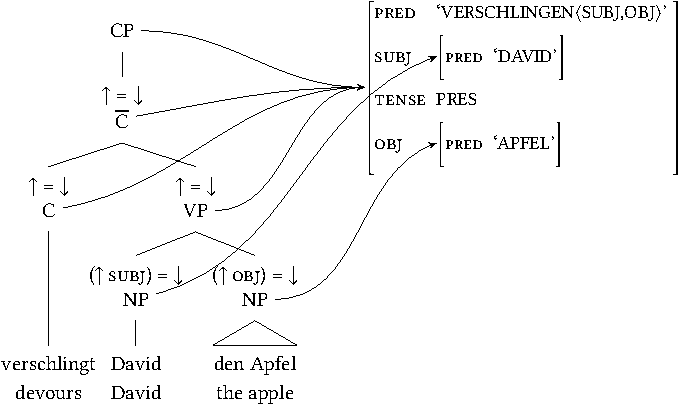
\includegraphics[width=.9\textwidth]{Figures/verschlingt-david-den-apfel-lfg-lsp-crop}

\bigskip

Analyse frei nach \citet[\page 41]{Berman2003a}.


}


\subsection{Lokale Umstellungen}

\frame{
\frametitle{Lokale Umstellungen}

\begin{itemize}
\item Zwei Möglichkeiten werden in der Literatur diskutiert:
      \begin{itemize}
      \item Umstellung von Argumenten aus einer Basiskonfiguration wie in GB\\
            (siehe \citew{Choi99a-u})
\pause
      \item direkte Ableitung über Phrasenstrukturregeln (siehe \citew{Berman96a-u,Berman2003a})
      \end{itemize}
\end{itemize}

}

\frame[shrink=15]{
\frametitle{Unterspezifikation des Kasus in der c-Struktur}

\begin{itemize}
\item Die Regel, die wir schon kennen, sagt nichts über den Kasus oder die grammatischen Funktionen
  der Elemente aus:
\ea
VP $\to$ (NP) (NP) (NP) (V)
\z
Wenn man die grammatische Funktion einer NP erst in Abhängigkeit von ihrem Kasus bestimmt, dann kann
  man mit der Regel in (\mex{0}) alle Anordnungen der Nominalphrasen ableiten.

\item \citet[\page 37]{Berman2003a} schlägt ähnliche Analyse vor:\\
\ea
      (\down {\sc case}) = ACC $\Rightarrow$ (\up \lfgobj)=\down{}
\z

%% Nee, denn das macht sie mit Spur.
%%
%%       Problem bei Fernabhängigkeiten, da Vorfeldelemente nicht unbedingt zur obersten f-Struktur
%%       beitragen.
%% \ea
%% Wen glaubst du, dass ich getroffen habe.
%% \z
%% Wenn hier \emph{wen} (\up \lfgobj)=\down{} ist, wird die f-Struktur für \emph{glauben} inkohärent.

%\item Brutale Lösung: Aufzählung aller Permutationen mit Kasus und f-Struktur-Annotation in den
%Phrasenstrukturregeln.
%
% Wen glaubst du, dass Peter seinen Freund belehrt, dass ich getroffen habe.
% Wenn man statt \up obj einen Regulären Ausdruck (\up COMP* \lfgobj) verwenden würde,
% Dann könnte wen zu belehren gehen und ihn zu getroffen
%
% Peter hat ihm versprochen, öfter zu helfen.
%
\end{itemize} 


}



\subsection{Fernabhängigkeiten und Funktionale Ungewißheit}

\subsubsection{Diskursfunktionen}


\frame{
\frametitle{Fernabhängigkeiten: Diskursfunktionen (I)}


\begin{itemize}
\item Beobachtung: die versetzte Konstituente (\emph{Chris} in
(\mex{1})) ist durch zwei Funktionen ausgezeichnet:
\ea
Chris, we think that David saw.
\z

  \begin{itemize}
  \item eine \blaubf{Argumentfunktion}, die kanonisch an anderer
  Stelle realisiert w\"urde\\
  (im Beispiel \textsc{obj} des Verbs \emph{saw}),
\pause
  \item eine besondere Hervorhebung des informationsstrukturellen
  Status in diesem Satzgef\"uge -- eine sog.\ \blaubf{Diskursfunktion}\\
  (im Beispiel \textsc{topic} des Matrixsatzes).
  \end{itemize}
\end{itemize}

}

\frame{
\frametitle{Diskursfunktionen (II)}

\begin{itemize}
\item Grammatikalisierte Diskursfunktionen: \textsc{topic} und \textsc{focus}\\
      (daneben wird \textsc{subj} als Default"=Diskursfunktion klassifiziert).
  \begin{itemize}
  \item Nur \textbf{grammatikalisierte} Diskursfunktionen werden auf
  f-Struktur markiert, also solche, die einem festen syntaktischen
  Mechanismus unterliegen und mit dem Rest der Syntax interagieren.

%%   (F\"ur die umfassende Repr\"asentation von informationsstrukturellen
%%   Eigenschaften wird in LFG eine separate Informationsstruktur
%%   angenommen.)
\pause
  \item Im Gegensatz zu den Argumentfunktionen werden die
  Diskursfunktionen \textsc{topic} und \textsc{focus} nicht lexikalisch subkategorisiert\\
 (unterliegen also nicht der \emph{Completeness}- und
  \emph{Coherence}-Bedingung)
\pause
  \item \textsc{topic} und \textsc{focus} werden 
%\"uber funktionale oder anaphorische Kontrolle 
  mit einer f-Struktur identifiziert,\\
  die eine Argument-Funktion tr\"agt.
  \end{itemize}
\end{itemize}

}

\frame{
\frametitle{Diskursfunktionen in der f-Struktur}
\smallframe

\eal
\ex Chris, we think that David saw.
\ex 
\lfgms{ pred & `think\sliste{ \lfgsubj, \comp }' \\
        topic & \rnode{topic}{\lfgms{ pred & `Chris' \\
                                   }}\\[4mm]
        subj & \lfgms{ pred & `pro'\\
                     }\\
        comp & \lfgms{ pred & `see\sliste{ \lfgsubj, \lfgobj }\\
                       subj & \lfgms{ pred & `David' \\
                                    }\\
                       obj  & \rnode{obj}{}\\
                     }\\
      }
\nccurve[ncurv=2.2]{topic}{obj}
\zl

\bigskip
Der Strich sagt: Der Wert von {\sc topic} ist mit dem von \textsc{comp obj} identisch.

Als Beschränkung: (\up  \textsc{topic})=(\up \textsc{comp obj})
}

\frame{
\frametitle{Verschiedene Einbettungstiefen (I)}

\eal
\ex Chris, we saw.
\ex 
\lfgms{ pred & `see\sliste{ \lfgsubj, \lfgobj }' \\
        topic & \rnode{topic}{\lfgms{ pred & `Chris' \\
                                   }}\\[4mm]
        subj & \lfgms{ pred & `pro'\\
                     }\\
        obj  & \rnode{obj}{}\\
      }
%\nodecurve[r]{topic}[r]{obj}{15em}
\nccurve[nodesepA=1pt,ncurv=2.2]{topic}{obj}
\zl

\bigskip

Als Beschränkung: (\up  \textsc{topic})=(\up \textsc{obj})
}


\frame{
\frametitle{Verschiedene Einbettungstiefen (II)}
\smallframe

\eal
\ex Chris, we think Anna claims that David saw.
\ex 
\scalebox{0.85}{%
\lfgms{ pred & `think\sliste{ \lfgsubj, \comp }' \\
        topic & \rnode{topic}{\lfgms{ pred & `Chris' \\
                                   }}\\[4mm]
        subj & \lfgms{ pred & `pro'\\
                     }\\
        comp & \lfgms{ pred & `claim\sliste{ \lfgsubj, \comp }\\
                       subj & \lfgms{ pred & `Anna' \\
                                   }\\
                       comp & \lfgms{ pred & `see\sliste{ \lfgsubj, \lfgobj }\\
                                      subj & \lfgms{ pred & `David' \\
                                                   }\\
                                      obj  & \rnode{obj}{}\\
                                    }\\
                     }\\
      }
%\nodecurve[r]{topic}[r]{obj}{15em}%
\nccurve[ncurv=2.2]{topic}{obj}
}
\zl

Als Beschränkung: (\up  \textsc{topic})=(\up \textsc{comp comp obj})
}

\frame{
\frametitle{Funktionale Ungewißheit}

\begin{itemize}
\item Die Beschränkungen sind c-Struktur-Beschränkungen:
\begin{tabular}{@{}ccc@{~=~}lc@{}}
CP & $\rightarrow$ & \multicolumn{2}{l}{\hspaceThis{(\up \textsc{topic})}XP} & C$'$ \\
 & &  (\up \textsc{topic}) & \down & \up=\down \\
 & &  (\up \textsc{topic}) & (\up \textsc{comp obj})\\
\end{tabular}

\pause
\item Wir haben aber auch andere Einbettungestiefen:

(\up  \textsc{topic})=(\up \textsc{obj})\\
(\up  \textsc{topic})=(\up \textsc{comp obj})\\
(\up  \textsc{topic})=(\up \textsc{comp comp obj})\\
\ldots

\pause
\item Die Generalisierung über diese Gleichungen ist:

(\up  \textsc{topic})=(\up \textsc{comp* obj})
\medskip

Dabei steht der `*' für beliebig viele Vorkommen von \comp.

\end{itemize}

}

\frame{
\frametitle{Disjunktionen und Variablen für grammatische Funktionen}


\begin{itemize}[<+->]
\item Im Deutschen kann nicht nur ein {\sc topic} im Vorfeld stehen,\\
      sondern auch ein \focus.
\item Man kann in LFG-Gleichungen auch Disjunktionen verwenden:

(\up  \textsc{topic$|$focus})=(\up \textsc{comp* obj})

\item Für \textsc{topic$|$focus} kann man einen eigenen Bezeichner einführen:\\
      {\sc df} steht für eine Disjunktion der Diskursfunktionen.


%% \begin{tabular}{@{}ccc@{~=~}lc@{}}
%% CP & $\rightarrow$ & \multicolumn{2}{l}{\hspaceThis{(\up \textsc{topic})}XP} & C$'$ \\
%%  & &  (\up \textsc{DF}) & \down & \up=\down \\
%%  & &  (\up \textsc{DF}) & (\up \textsc{comp* GF})\\
%% \end{tabular}

\end{itemize}

}

\subsection{Zusammenfassung}

\frame{
\frametitle{Zusammenfassung}

\begin{itemize}
\item LFG ist unifikationsbasiert, arbeitet mit Merkmalsstrukturen und PSG-Regeln
\item Grammatische Funktionen sind Primitive der LFG,\\
      sie sind nicht strukturell definiert (wie in der GB)
\item LFG ist lexikalistisch. Valenzänderungen wie bei Passivierung erfolgen im Lexikon
mittels lexikalischer Regeln.
\end{itemize}

}
